 \documentclass{article}

% Call the style package
\usepackage{fun3style}
\usepackage[shortlabels]{enumitem}
\usepackage{multirow}
\usepackage{graphicx}
\usepackage{float}
\usepackage{forest}
\usepackage{csvsimple}
    
\title{Multi-Agent Systems: Final Homework Assignment}
\author{Neil Mizzi Student No:(2674737) \\ MSc. Artificial Intelligence -- Vrije Universiteit van Amsterdam}
\date{6 January 2020}

\restylefloat{table}

\begin{document}
\maketitle

\section{Multi-Armed Bandits}
\subsection{Thompson Sampling for a single Bandit}
\subsubsection{Beta-Density Sampling}
In this section, we demonstrate the four properties of the beta distribution. The Beta distribution is a probability distribution which takes $\alpha$ and $\beta$ values and returns a value in the range $0 \leq x \leq 1$, dependent on the values of $\alpha$ and $\beta$. The Beta distribution is defined as follows:

\begin{equation}
    B(x; \alpha, \beta) = 
    \frac{(\alpha + \beta -1!}{(\alpha -1)!(\beta-1)!}x^{\alpha - 1}(1-x)^{\beta -1}
\end{equation}
Where  $0 \leq x \leq 1$

The four properties associated to this distribution are as follows:
\begin{enumerate}
    \item if $\alpha = \beta = 1$, then we have a uniform distribution
    \item if $\alpha = \beta \neq 1$, then we have a symmetric distribution. A symmetric distribution is one where the values of the samples are concentrated towards the upper and lower limits, respectively.
    \item if $\alpha > \beta$, then the distribution is concentrated towards the upper limit (i.e. the sample has a high chance of being close to the value of 1, for $0 \leq x \leq 1$)
    \item if $\alpha$ and $\beta$ both have large values, then the distribution is more concentrated. By concentration, we mean that the distribution has a low variance.
\end{enumerate}
//TODO Look up how to fix figure when getting internet
\begin{figure}
	\centering
	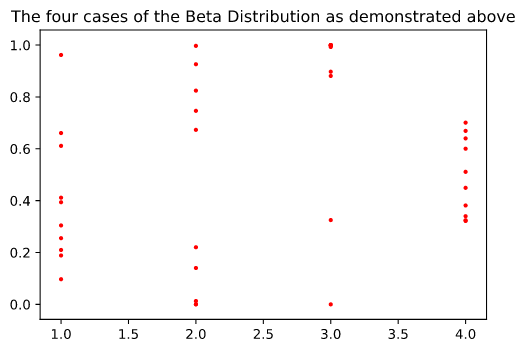
\includegraphics{test_results/beta_distributions}
	\label{fig1_betaDistribution}
	\caption{Distribution of the four cases mentioned previously}
\end{figure}

In Figure \ref{fig1_betaDistribution}, we sample 20 values with the following properties:
\begin{enumerate}
	\item The first distribution is a uniform one, i.e. $\alpha = \beta = 1$
	\item The second distribution picks a random value such that $\alpha = \beta \neq 1$, in the range $0 \leq \alpha, \beta \leq 1$
	\item The third distribution picks values such that $0 \leq \beta \leq \alpha \leq 1$
	\item The final distribution has been set fixed, such that $\alpha = 5$ and $\beta = 6$
\end{enumerate}

We can note from figure \ref{fig1_betaDistribution} that the above properties do hold. It is important to note that the $\theta$ value, where $\theta = \frac{\alpha}{\beta}$, makes an impact of where the values of the beta distributions are concentrated. In the next section, we will note that the higher the theta value, the values of the distribution are more concentrated towards the upper bound.

\subsubsection{Thompson Update Rule}
The Thompson Update rule is one of the basis for Thompson Sampling rule for a multi-armed bandit algorithm. The rule checks for a Bandit reward at every iteration, and updates the $\alpha]$ and $\beta$ values accordingly. In a scenario where $k > 1$, this will be able to demonstrate a balance of exploration and exploitation. \\ The update rule can be informally defined as follows:

\begin{itemize}
	\item Initialise $\alpha = \beta = 1$, to start off with a uniform distribution
	\item Retrieve a bandit sample such that $r = 0$ or $r = 1$. The value of $r$ is determined such that given a beta sample $x$ and an unknown random probability $p$, then $r = 1$ if $x > p$, else $r = 0$
	\item$\alpha$ and $\beta$ are updated such that:
\end{itemize}
\begin{center}
	$\alpha \leftarrow \alpha + r$, $\beta \leftarrow \beta + (1-r)$
\end{center}
//TODO Insert Figures as subplots
In figures (insert figure refs here), we test the update rule for 10000 iterations. One thing of note is that the distribution does not always peak to the same value. 

In the first test case, indicated by (insert test1 ref here), the $\theta$ value is considerably high, indicating that the $\alpha$ value has been growing much more than the $\beta$ value, therefore resulting in a distribution mean which peaks towards the value of $1$.

In the second test case, indicated by (insert test2 ref here), the $\theta$ value floats just above $1$, indicating that both $\alpha$ and $\beta$ are being incremented at a steady pace, with $\alpha$ being slightly higher. This results in a mean distribution of approximately $0.6$.

In the last test case, indicated by (insert test3 ref here), $\theta \leq 1$. This indicates that the $\beta$ value has taken priority, indicating that there are more bandits such that the returned reward is $r=0$, and therefore resulting in a relatively low distribution mean of approximately $0.3$.

One common thing to note in the above test cases is that the standard deviation (and subsequently also the variance) of the distribution has considerably dropped in the beginning of application of the update rule. This indicates that Rule 4 of the beta distribution (where high values of $\alpha$ and $\beta$ results in a more peaked distribution) does indeed hold, no matter the values of $\alpha$ and $\beta$, therefore determining at an early stage if a bandit is successful or not.


\subsection{Thompson Sampling for a 2-armed Bandit}
Yet more Memes
\section{Reinforcement Learning: Cliff Walking}


\end{document}